Das Template des Signals wird mit Hilfe der Information der Monte Carlo Simulation erstellt.
Dabei wird ausgenutzt, dass in der Simulation bekannt ist, welchen Ursprung welches Teilchen hat und welches Teilchen auf das EMCal trifft.
Dadurch wird ermöglicht, genau bestimmen zu können, ob ein Teilchen aus dem Zerfall eines $\pi^{0}$ oder einem anderen Prozess stammt und ob es sich dabei um ein Photon, ein konvertiertes Elektron oder Positron, oder ein anderes Teilchen handelt.
\begin{figure}[tp]
\centering
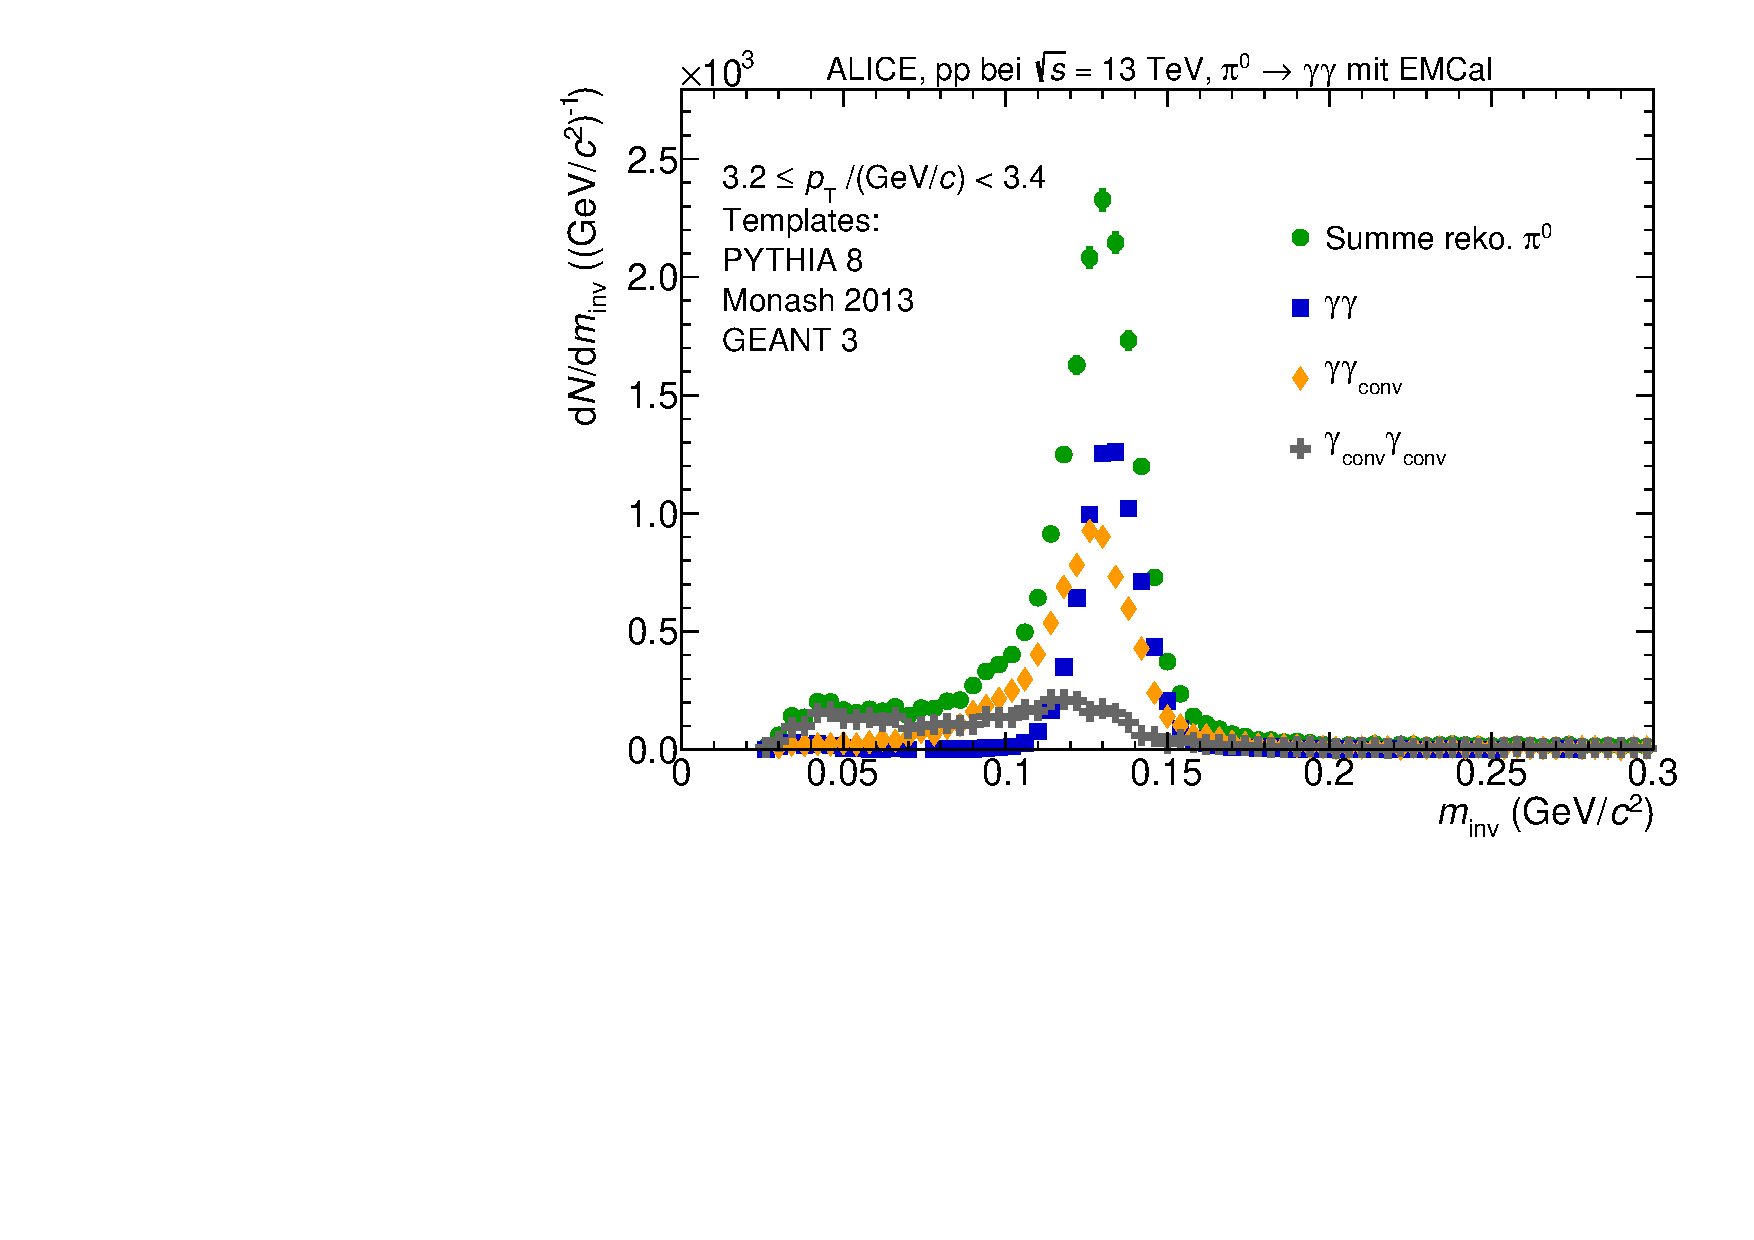
\includegraphics[width=.75\linewidth]{PeakTemplateMotivation10_Data_2016.pdf}
\caption{Template des Signals (grün) mit seinen drei Teilkomponenten.
Diese bestehen aus Kombinationen mit zwei Photonen (blau), einem Photon und einem Konversionselektron oder Konversionspositron (gelb) und zwei unterschiedlichen Konversionselektronen oder Konversionspositronen (grau).}
\label{fig:SigTemp}
\end{figure}
\newline
Abbildung \ref{fig:SigTemp} zeigt die Anzahl \textit{Clusterpaare} von Teilchen, die aus dem Zerfall eines einzelnen $\pi^{0}$ kommen in, was aus der Simulation bekannt ist, in grün. 
Zusätzlich wurden die Komponenten eingezeichnet, in die sich das Signal teilen lässt.
Die Komponenten setzen sich aus drei möglichen Kombinationen von \textit{Clustern} zusammen.
Zum einen aus \textit{Clustern} aus Photonen, in der Abbildung als $\gamma$ bezeichnet, und zum anderen aus \textit{Clustern} aus einem Elektron oder Positron, die durch die Konversion  eines Photonen entstanden sind.
Letztere werden in der Abbildung durch $\gamma_\text{conv}$ symbolisiert.
\newline
In blau sind die Kombinationen aus zwei Photonen ($\gamma\gamma$) dargestellt, in gelb die Kombination aus Photon und Elektron oder Positron ($\gamma\gamma_\text{conv}$) und in grau die Kombination aus Konversionselektron oder Konversionspositron miteinander ($\gamma_\text{conv}\gamma_\text{conv}$).
Diese beiden Anteile wurden vorher zusammengefasst als Konversionsanteil.
\newline
Die Abbildung zeigt außerdem, wie zuvor angesprochen, dass bis $m_\text{inv}>0\,05 \text{ GeV}/c^{2}$ Signal vorliegt.
Der Anteil des Signals um diese invariante Masse besteht hauptsächlich aus zwei Teilchen aus einer Photonkonversion.
Genau dieser Teil des Signals wird nicht durch die Standardmethode berücksichtigt.
Durch das Berücksichtigen in der Analyse mit Hilfe der Templates kann ein größerer Anteil des Signals gezählt werden.
Deshalb wird eine geringere statistische Unsicherheit erwartet.